\documentclass[aps, 10pt, preprintnumbers,prd, amsmath,amssymb,twocolumn,notitlepage]{revtex4} %, ,10pt
%\documentclass[aps, 10pt, preprintnumbers,prd, amsmath,amssymb,notitlepage]{revtex4} %, ,10pt
\usepackage{graphicx}% Include figure files latexsym,array,enumerate,letter,numbers,twocolumn
%\usepackage{dcolumn}% Align table columns on decimal point
\usepackage{bm}% bold math
\usepackage{amssymb}
\usepackage{subfigure}
\usepackage{epsfig}
%\usepackage{slashed}
\usepackage{color}
%\usepackage{cite}
\usepackage{mathtools}
\usepackage{cases}
\usepackage{booktabs}
\usepackage{amsmath}
%\usepackage{subcaption}

\usepackage[
colorlinks=true,
filecolor=black,
anchorcolor=blue,
linkcolor=blue,
citecolor=cyan, %red,
urlcolor=cyan,
linktocpage=true,
plainpages=false,
breaklinks=true,
pdfstartview=FitH
]{hyperref}

\def\cd{\color[rgb]{0.00,0.50,0.25}} %delete
\def\cm{\color[rgb]{0.00,0.60,0.00}} %modify
\def\cn{\color[rgb]{0.80,0.00,0.40}} %
 
\def\m{{\cm\mu_0}}
\def\e{{\cm\epsilon_0}}


\newcommand{\nn}{\nonumber}
\newcommand{\kbh}{k_{\r{bh}}}
\newcommand{\sbh}{\sigma_{\r{bh}}}
\newcommand{\mbh}{m}
\newcommand{\neff}{N_{\rm{eff}}}
\newcommand{\dneff}{\Delta N_{\rm{eff}}}
\newcommand{\ms}{m_{\odot}}
\newcommand{\fbh}{f_{\r{bh}}}
\newcommand{\rd}{\r{d}}
\DeclareRobustCommand{\Eq}[1]{Eq.~(\ref{#1})}
\DeclareRobustCommand{\Fig}[1]{Fig.~\ref{#1}}

\newcommand{\ps}{P_{\mathcal{R}}}
\def\di{\mathrm{d}}

\def\eps{\epsilon}
%\def\d{\partial}
\def\l{\left(}
\def\r{\right)}
\def\la{\langle }
\def\ra{\rangle }



\newcommand{\ck}[1]{\textcolor{blue}{#1}}
\newcommand{\ckk}[1]{\textcolor{red}{#1}}
\newcommand{\vev}[1]{\left<{#1}\right>}
\newcommand{\bra}[1]{\left|{#1}\right>}
\newcommand{\ket}[1]{\left<{#1}\right|}


\newcommand{\E}{\mathbf{E}}
\newcommand{\B}{\mathbf{B}}
\newcommand{\J}{\mathbf{J}}
\newcommand{\Mpl}{M_{\rm Pl}}
\newcommand{\n}{\mathbf{n}}

\newcommand{\ab}{\alpha \beta}
\newcommand{\mn}{\mu \nu}
\newcommand{\rs}{\rho \sigma}
\newcommand{\hmn}{h_{\mu \nu}}
\newcommand{\TT}{\text{TT}}
\newcommand{\jeff}{j_\text{eff}}
\newcommand{\hnorm}{h_0}
\newcommand{\order}[1]{\mathcal{O}{(#1)}}
\newcommand{\nl}{\nonumber \\}
\newcommand{\w}{\omega}
\newcommand{\wg}{\omega_g}
\newcommand{\lamg}{\lambda_g}
\newcommand{\tTT}{t_{_\text{TT}}}
\newcommand{\xTT}{x_{_\text{TT}}}
\newcommand{\yTT}{y_{_\text{TT}}}
\newcommand{\zTT}{z_{_\text{TT}}}
\newcommand{\UTT}{U_{_\text{TT}}}
\newcommand{\jTT}{j_{_\text{TT}}}
\newcommand{\FTT}{F_{_\text{TT}}}
\newcommand{\fTT}{f_{_\text{TT}}}
\newcommand{\grad}{\nabla}

\newcommand{\jveff}{\boldsymbol{j}_\text{eff}}
\newcommand{\jvhat}{\hat{\jv \, }}
\newcommand{\jplus}{\jvhat_{\hspace{-0.1 cm} +}}
\newcommand{\jcross}{\jvhat_{\hspace{-0.1 cm} \times}}
\newcommand{\jpc}{\jvhat_{\hspace{-0.1 cm} +, \times}}

\newcommand{\emu}{\hat{\mathbf{e}}_\mu}
\newcommand{\enu}{\hat{\mathbf{e}}_\nu}
\newcommand{\erho}{\hat{\mathbf{e}}_\rho}
\newcommand{\ephi}{\hat{\mathbf{e}}_\phi}
\newcommand{\ez}{\hat{\mathbf{e}}_z}
\newcommand{\ex}{\hat{\mathbf{e}}_x}
\newcommand{\ey}{\hat{\mathbf{e}}_y}
\newcommand{\rv}{\mathbf{r}}
\newcommand{\vv}{\mathbf{b}}
\newcommand{\jv}{\mathbf{j}}
\newcommand{\rvp}{\mathbf{r'}}
\newcommand{\Rv}{\mathbf{R}}
\newcommand{\al}{S_\text{\scriptsize loop}}
\newcommand{\at}{S_\text{\scriptsize toroid}}
\newcommand{\rl}{\rho_\text{\scriptsize loop}}
\newcommand{\rt}{\rho_\text{\scriptsize max}}
\newcommand{\rmi}{\rho_\text{\scriptsize min}}
\newcommand{\bmax}{B_{\text{max}}}

\newcommand{\be}{\begin{equation}}
\newcommand{\ee}{\end{equation}}
\newcommand{\bea}{\begin{equation}\begin{aligned}}
\newcommand{\eea}{\end{aligned}\end{equation}}
\newcommand{\ga}{g_{a\gamma\gamma}}
\newcommand{\bE}{\mathbf{E}}
\newcommand{\bB}{\mathbf{B}}
\newcommand{\bP}{\mathbf{P}}
\newcommand{\bM}{\mathbf{M}}
\newcommand{\bk}{\mathbf{k}}
\newcommand{\bU}{\mathbf{U}}
\newcommand{\bV}{\mathbf{V}}
\newcommand{\rhoDM}{\rho_{\scriptscriptstyle \textrm{DM}}}
\newcommand{\PBH}{{\scriptscriptstyle \textrm{PBH}}}
\newcommand{\hTT}{h^{\scriptscriptstyle \textrm{TT}}}
\DeclareRobustCommand{\r}[1]{{\rm #1}}

\newcommand{\xv}{{\bf x}}
\newcommand{\Vcav}{V_\text{cav}}


%math symbols
\newcommand{\curl}{\nabla\times}

%math symbols
%\newcommand{\curl}{\nabla\times}
\begin{document}

\title{High Frequency Gravitational Implications from the NANOGrav 15 Year Data}
\author{Junsong Cang$^{1}$}
\email{cangjunsong@outlook.com}
\author{Yu Gao$^{2}$}
\email{gaoyu@ihep.ac.cn}
\author{Yi-ming Liu$^{3}$}
\email{your@email,\& please check affiliations}
\author{Sichun Sun$^{3}$}
\email{sichunssun@bit.edu.cn}


\affiliation{$^1$ School of Physics, Henan Normal University, Xinxiang, China}
\affiliation{$^{2}$Key Laboratory of Particle Astrophysics, Institute of High Energy Physics,
Chinese Academy of Sciences, Beijing 100049, China}
\affiliation{School of Physics, Beijing Institute of Technology, Beijing, 100081, China}


\begin{abstract}
\ckk{Message from JSC:
Please do not edit this draft at the moment as it is being edited locally on my computer because my overleaf crashes all the time.
The finished version will be uploaded before the end of this weekend.
}
\end{abstract}

\maketitle

\section{Introduction}

Enthusiasm in primordial black holes (PBHs)~\cite{Zeldovich:1967lct,Carr:1974nx} has grown immensely after the LIGO discovery of gravitational wave signals~\cite{} in agreement with merger events of black holes above stellar masses. Primordial black holes can originate from the collapse of large density fluctuations in the early Universe. If produced in abundance, such PBHs are under extensive searches for their own astrophysical signals, see Ref.~\cite{Carr:2021bzv} for a recent review. The early process of over-density collapse is also predicted to release scalar-induced gravitational waves (SIGW)~\cite{}, which penetrate the hot environment of the early Universe, and offer a glimpse at valuable information of early fluctuations at late-time gravitational wave detectors.

{\color{blue}
The primordial black hole can be supermassive, to generate gravitational waves from the mergers directly. In the case of the scalar-induced gravitational waves(SIGW), the associated PBH produced in this case is a couple of orders below solar mass, and the mergers of such light PBH produced a gravitational wave signal around Mhz. Since the endeavor of the whole gravitational wave frequency spectrum searches has begun, with various proposals already in Mhz-Ghz band\cite{}, it is intriguing to link the ultra-low NanoHz gravitational waves to the ultra-high frequency gravitational searches. We may call it a multi-messager task in the frequency spectrum space.
}

In recent years, several Pulsar Timing Array (PTA) observatories including NANOgrav~\cite{NANOGrav:2020bcs}, Parkes PTA~\cite{Goncharov:2021oub}, European PTA~\cite{Chen:2021rqp} and a joint study ~\cite{Antoniadis:2022pcn} reported strong indication of a common-spectrum process in the 1-10 nano-Hertz waveband. 
These observations incited several studies on a potential signal from supermassive black holes~\cite{Middleton:2020asl}, or from more cosmological origins, such as phase transition~\cite{Bian:2020urb,NANOGrav:2021flc,Xue:2021gyq,Wang:2022wwj} and axion topological defects~\cite{Wang:2022rjz,Ferreira:2022zzo}, etc. Continued PTA observations are expected to verify the robustness of the earlier claim. 

\ck{cjs: add - $\ps$ well constrained at large scales but can potentially have large amplitude at small scales and thereby producing SIGW for NG15}

In the latest release of PTA data, NANOgrav XXX year-data~\cite{}... The Chinese PTA reported a $4.6\sigma$ detection of quadrupolar correlation~\cite{Xu_2023} that indicates for a cosmic origin of the GW signal. ... In case of SIGW from overdensity collapse, a GW signal at NANOgrav's nHz frequency generally requires a power spectrum $P(k)$ with large fluctuations at the scale of $k\sim 10^{6-8}$ Mpc$^{-1}$. Compared to other power-spectrum constraints like the large-scale structure ($k<$Mpc$^{-1}$), the cosmic microwave background ($k< 10^{-XX}$ Mpc$^{-1}$)~\cite{Hunt:2015iua}, scale-insensitive $N_{\rm eff}$~\cite{PLK2015,Cang:2022jyc} and big-bang nucleosynthesis~\cite{Kohri:2018awv,Inomata:2018epa} bounds, this is a comparably small  fluctuation scale, where the power spectrum is largely unconstrained by other experiments~\cite{}. 

In this paper, we adopt a log-normal power spectrum in the XXX model, and we show the latest NANOgrav result is in cosistency with ... We also discuss the abundance of the associately produced PBHs in the same process.



%in the  that behave like an extra radiation component,
%thus contributing to the relativistic degrees of freedom ($\neff$).
%We show that the cosmological constraints on $\neff$ can be used to pose stringent limits on PBHs created from this particular scenario as well as the relevant small-scale curvature perturbation ($\ps(k)$).

\section{Production of SIGW and PBH}
We consider a log-normal model for primordial curvature perturbation $\ps$,
\be
\ps
=
\frac{A}{\sqrt{2 \pi \Delta^2}}
\exp
\left[
-\frac{(\ln k/k_*)^2}{2\Delta^2}
\right]
\ee
where $A,\ k_*$ and $\Delta$ are model parameters,
which describe the amplitude,
peak location and the width of $\ps$ respectively.
Upon horizon crossing,
$\ps$ will modify the radiation quadruple moment and generate SIGW at second order,
whose energy density today is given by~\cite{Cang:2022jyc,Ando:2018qdb,Kohri:2018awv,Inomata:2018epa}

\be
\begin{aligned}
\frac{{\rm d}\Omega_{\rm SIGW}}{{\rm d}\ln k}
& = 
0.29~
\Omega_{\r{r}}
\left(
\frac{106.75}{g_{\ast}}
\right)^{1/3}
\\
&
\ \ \ \ 
\times
\int^\infty_0 dv \int^{1+v}_{|1-v|} du \left[ \frac{4v^2-(1-u^2+v^2)^2}{4u^2v^2}\right]^2
\\
&\ \ \ \  \times \left(\frac{u^2+v^2-3}{2 u v}\right)^4 F(u,v) \ps(kv)\ps(ku),
\end{aligned}
\ee
\be
\begin{aligned}
F(u,v)
&=
\left( \ln\left| \frac{3-(u+v)^2}{3-(u-v)^2}\right|-\frac{4 u v}{u^2+v^2-3}\right)^2
\\
&
+
\pi ^2 \Theta \left(u+v-\sqrt{3}\right)
,
\end{aligned}
\ee
here $\Omega_\r{SIGW} \equiv \rho_\r{SIGW}/\rho_\r{cr}$ is the density fraction of SIGW,
$\Omega_{\rm r}=9.1 \times 10^{-5}$ is current radiation density fraction assuming massless neutrinos,
$g_*$ is the total degree of freedom for massless particles when the mode $k$ enters horizon ($k=aH$)~\citep{KolbTurner1990,Wallisch:2018rzj}.
The frequency of SIGW is related to the wavenumber $k$ via[],
\be
f = 1.546 \times 10^{-15}\left(\frac{k}{\r{Mpc^{-1}}}\right) \r{Hz}
\ee

In addition to emitting SIGW,
sufficiently large $\ps$ will also generate overdense regions that can gravitationally collapse into PBHs.
The mass of PBH formed in this process is related to wavenumber $k$ via~\cite{Cang:2022jyc,Carr:2009jm,Nakama:2016gzw,Ozsoy:2018flq,Chen:2021nio},
\be
\mbh
=
2.43 \times 10^{-4}
\left(
\frac{\gamma}{0.2}
\right)
\left(
\frac{g_{\ast}}{106.75}
\right)^{-1/6}
\left(
\frac{k}{10^8\rm Mpc^{-1}}
\right)^{-2}
\ms,
\label{k2m_relation}
\ee
here $\gamma$ is the collapse efficiency,
for which we adopt a typical value of $\gamma = 0.2$ following
~\cite{
Carr:2009jm,
Ozsoy:2018flq,
Chen:2021nio}.
The corresponding distribution of PBH abundance is given by~\cite{Ozsoy:2018flq, Carr:2020xqk, Young:2014ana,Ozsoy:2018flq,1975ApJ...201....1C},
\be
\begin{aligned}
\psi
&\equiv
\frac{\r{d}\fbh}{{\rm d} \ln \mbh}
\\
&=
0.28
\left(
\frac{\beta}
{10^{-8}}
\right)
\left(
\frac{\gamma}{0.2}
\right)^{3/2}
\left(
\frac{g_{\ast}}{106.75}
\right)^{-1/4}
\left(
\frac{\mbh}{\ms}
\right)^{-1/2}
,
\label{9876tyuuyt}
\end{aligned}
\ee
where $\fbh \equiv \rho_\r{bh}/\rho_\r{dm}$ is the fraction of DM made of PBHs,
and
\be
\beta (\mbh)
\simeq
\sqrt{
\frac{2 \bar{\sigma}^2}
{\pi \delta_{\rm c}^2}
}
\r{exp}
\left(
-\frac{\delta_{\rm c}^2}{2 \bar{\sigma}^2}
\right),
\label{7865rt54321qw}
\ee
\be
\bar{\sigma}^2
(\mbh)
=
\frac{16}{81}
\int
\r{d}
\ln
k'\,
\left(
\frac{k'}{k}
\right)^4
\ps
(k')
W^2\left(\frac{k'}{k} \right),
\label{8765rfgrtf}
\ee
here $\delta_\r{c}$ is the threshold for gravitational collapse,
for which we adopt 0.45 following [].
$W(x)$ is a window function, 
which we use $\exp(-x^2/2)$~\citep{Ozsoy:2018flq,Chen:2021nio}.

In practice,
we find that the distribution calculated from \Eq{9876tyuuyt} can be well fit by a log-normal profile~\cite{Cang:2022jyc},
\be
\psi
=
\fbh
\frac{1}{\sqrt{2 \pi} \sbh}
\exp
\left[
-
\frac{\r{ln}^2(\mbh/m_{\r{c}})}
{2 \sbh^2}
\right]
,
\label{dshiuy65}
\ee
where $m_\r{c}$ and $\sigma_\r{bh}$ are peak and width of the distribution respectively.
For convenience,
in what follows we will parameterise our PBH distribution using \Eq{dshiuy65}.

%Note that it's often convenient to describe PBH distribution via number density rather than mass density in \Eq{dshiuy65},
%\be
%\begin{aligned}
%\Psi
%&\equiv
%\frac{1}{n_\r{bh}}
%\frac{\rd n_\r{bh}}{\rd \ln m}
%\\
%&=
%\frac{\left<\mbh\right>}{\mbh}
%\frac{1}{\sbh \sqrt{2 \pi}}
%\exp
%\left[
%-
%\frac{\r{ln}(\mbh/m_{\r{c}})^2}
%{2 \sbh^2}
%\right]
%\end{aligned}
%\ee
%
%\be
%\begin{aligned}
%\left<
%\mbh
%\right>
%&\equiv
%\frac{\rho_{\r{bh}}}
%{n_{\r{bh}}}
%\\
%&=
%\left[
%\frac{1}{\sqrt{2 \pi} \sbh}
%\int
%\frac{\rd \ln \mbh}
%{\mbh}
%\exp
%\left[
%-
%\frac{\r{ln}(\mbh/m_{\r{c}})^2}
%{2 \sbh^2}
%\right]
%\right]^{-1}
%\end{aligned}
%\ee

\section{GW from PBH merger}
We follow the procedure detailed in [xxxx] to compute the GW from merging PBH binaries and we describe the key ingredients here.
The comoving merger rate $R$ of a pair of PBHs with mass $m_1$ and $m_2$ is given by,
\be
\begin{aligned}
\frac{\rd R}{\rd m_1 \rd m_2}
&\simeq
\frac{1.6 \times 10^6}
{\r{Gpc^3 yr}}
\fbh^{-\frac{21}{37}}
\eta^{-\frac{34}{37}}
\left(
\frac{M}{m_\odot}
\right)^{-\frac{32}{37}}
\\
&
\times
\left(
\frac{t}{t_0}
\right)^{-\frac{34}{37}}
S
\psi(m_1)
\psi(m_2)
\end{aligned}
\ee
where 
$M = m_1 + m_2$,
$\eta = m_1 m_2 / M^2$,
$t$ is the time of merger,
$t_0 = 13.8 \r{Gyr}$ is the current age of the Universe.
$S$ is a suppression factor which takes the form,
\be
S = S_1 \times S_2
\ee

\be
\begin{aligned}
S_1
&=
\frac{\r{e}^{-\bar{N}(y)}}
{\Gamma(21/37)}
\int \rd v
v^{-\frac{16}{37}}
\exp
\left[
-
\phi
-
\frac{3 \sigma^2_\r{M} v^2}
{10 \fbh^2}
\right]
\end{aligned}
\ee

\be
S2 \simeq
\r{min}
\left[
1,
1.96
\times
10^{-3}
x^{-0.65}
\exp
\left(
0.03
\ln^2
x
\right)
\right]
\ee
where 
$
F(z)
=
_1F_2
(-1/2,3/4,5/4;-9z^2/16)
-1
$,
$_1F_2$ is the generalised hypergeometric function,
$\sigma_\r{M} \simeq 0.004$,
$x = (t/t_0)^{0.44} \fbh$ and the rest of the terms read,
\be
\phi
=
\frac{
\bar{N}(y)
\left<
m\right>
}
{\fbh}
\int
\frac{\rd \mbh}{\mbh}
\psi(m)
F
\left(
\frac{M}
{
\left<
m
\right>
}
\frac{v}
{\bar{N}(y)}
\right)
\ee

\be
\bar{N}(y)
\simeq
\frac{M}
{\left<m\right>}
\frac{\fbh}
{\fbh + \sigma_\r{M}}
\ee

\be
\begin{aligned}
\left<
m
\right>
&\equiv
\fbh
\left[
\int \rd \ln\mbh
\ 
\frac{\psi}{\mbh}
\right]^{-1}
\\
&=
m_\r{c}
\r{e}^{-\sbh^2/2}
\end{aligned}
\ee
the energy density per $\ln f$ interval can be expressed as[1707],
\be
\frac{{\rm d}\Omega_{\rm MGW}}{{\rm d}\ln \nu}
=
\frac{f}{\rho_\r{cr}}
\int \frac{\rd z \rd R}
{(1+z)H}
\frac{\rd E_\r{GW}(f_\r{r})}
{\rd f_\r{r}}
\ee
here $f_\r{r}$ is the redshifted source frequency,
$\rd E_{\r{GW}}/\rd f_{\r{r}}$ describes the energy spectrum of PBH merger,

\be
\begin{aligned}
\frac{\rd E_\r{GW}(f_\r{r})}
{\rd f_\r{r}}
&=
(\pi G)^{2/3}
M^{5/3}
\eta
\\
&
\times
\left\{
\begin{array}{l}
f^{-1/3}_\r{r}
,
\ \ \ \ \ \ \ \ \ \ \ \ \ \ \ \ \ \ \ \ \ \ \ \ \ \ \ \  f_\r{r} < f_1\\
\\
\frac{f^{2/3}_\r{r}}
{f_1}
,
\ \ \ \ \ \ \ \ \ \ \ \ \ \ \ \ \ \ \ \ \  \ \ \ \ \ \  f_1 \le f_\r{r} < f_2\\
\\
\frac{f^2_\r{r}}
{f_1 f_2^{4/3}}
\frac{f_4^4}
{\left(
4(f_\r{r}
-f_2
)^2
+
f_4^2
\right)^2
}
,  
\ \ \ \ \  f_2 \le f_\r{r} < f_3\\
\end{array}
\right.
\end{aligned}
\label{eqdsfgr89inja}
\ee
here $f_i = (a_i \eta^2 + b_i \eta + c_i)$,
the polynomial coefficients $a_i,\ b_i, c_i$ are taken from [xxxx] and we list them all here in 
Tab.\ref{t456h3wedfghsa}.
\begin{table}[htp]
\begin{tabular}{c|ccc}
\hline
  & a & b & c\\
\hline
$f_1$ & $2.9740 \times 10^{-1}$ & $\ \ \ 4.4810 \times 10^{-2}$ & $\ \ \ 9.5560 \times 10^{-2}$\\
$f_2$ & $5.9411 \times 10^{-1}$ & $\ \ \ 8.9794 \times 10^{-2}$ & $\ \ \ 1.9111 \times 10^{-1}$\\
$f_3$ & $8.4845 \times 10^{-1}$ & $\ \ \ 1.2848 \times 10^{-1}$ & $\ \ \ 2.7299 \times 10^{-1}$\\
$f_4$ & $5.0801 \times 10^{-1}$ & $\ \ \ 7.7515 \times 10^{-2}$ & $\ \ \ 2.2369 \times 10^{-2}$\\
\hline
\end{tabular}
\caption{
Polynomial coefficients for characteristic frequencies $f_1,\ f_2,\ f_3$ and $f_4$ in 
\Eq{eqdsfgr89inja}.
}
\label{t456h3wedfghsa}
\end{table}

\section{Data Analysis}
We used PTA datasets from NanoGrav[], IPTA[] and PPTA[] to find the credible region for PBHs that will be used for subsequent merger GW calculation.
Our log-likelihood takes the form,
\be
\ln \mathcal{L}
=
-\frac{1}{2}
\sum_{i}
\frac{(x_i - u_i)^2}{\sigma_i^2}
\label{dshf3765rghfdv}
\ee
here the index $i$ denotes frequency,
$x$ is $\Omega_\r{GW}$ for our model,
$u$ is the measured median for $\Omega_\r{GW}$,
$\sigma$ is the error bar for $\Omega_\r{GW}$,
which equals $\sigma_T$ for $x>u$ and $\sigma_L$ otherwise.
$\sigma_T$ and $\sigma_L$ are upper and lower error bars respectively.
For convenience,
we follow~\cite{Franciolini:2023pbf} and estimate the signal median and error bars for each experiment directly using the $\Omega_\r{GW}$ posterior from [],
and we have checked that our results (when using NG15 data only) agrees very well with that shown in~\cite{Franciolini:2023pbf} and [NG15 new physics].

Note that as a form of dark radiation,
the extra energy budget from SIGW will also change the effective degree of relativistic degrees of freedom $\neff$,
which has been constrained by datasets from CMB, BAO and BBN (CBB) to~\cite{Cang:2022jyc}[PLK],
\be
\dneff
\equiv
\neff - N_\r{eff, SM}
\le
0.175
,\ 95\%\ \r{C.L.}
\label{dsfhi38r767fdg}
\ee
here $N_\r{eff, SM} = 3.046$ is the value of $\neff$ predicted by the standard model of particle physics[],
and $\Omega_\r{GW}$ is related to $\dneff$ by~\cite{Cang:2022jyc},
\be
\neff
=8.3 \times 10^4 \,\Omega_{\r{GW}},
\label{dsvuytdui}
\ee
As shown in the $\dneff$ posterior in \Fig{e2ftssaasadwu},
the $\dneff$ set by GW data alone gives violates the CBB constrains above.
Thus to accomondate the CBB $\neff$ limits,
we added a prior of $\dneff < 0.175$ to our inference.
Additionally we also restrict our inference to $\fbh \in [10^{-20}, 1]$,
such that PBH does not exceed the DM density ceiling while still has physically meaningful abundance for appreciable merger GW production.

We sampled the likelihoods in \Eq{dshf3765rghfdv} using the {\tt multinest} sampler[].
We considered a total of 3 inference settings:
\begin{itemize}
\item {\bf GW}: Use PTA GW data alone.
\item {\bf GW + $\dneff$}: Use PTA GW data and CBB $\dneff$ limits in \Eq{dsfhi38r767fdg}.
\item {\bf GW + $\dneff$ + PBH}: Use PTA GW data and CBB $\dneff$ limits along with the prior of $\fbh \in [10^{-20}, 1]$.
\end{itemize}

Tab.\ref{tabd76543wedfghsa} summarises the parameter prior ranges in our inference.
\Fig{e2ftssaasadwu} shows the marginalised results of our fitting,
the left panel shows the posterior for our model parameters and the derived $\dneff$,
the right panel shows the posterior for PBH parameters $\fbh$, $m_\r{c}$ and $\sigma_\r{bh}$.

\begin{table}[htp]
\begin{tabular}{c|c}
\hline
Parameters & Prior range\\
\hline
$\log_{10}A$& [-1.8, 0]\\
$\log_{10}(k_*/\r{Mpc^{-1}})$& [6.8, 9]\\
$\Delta$& [0, 4]\\
\hline
$\Delta N_\r{eff}$&  $\le 0.175$\\
$\log_{10}f_\r{bh}$& [-20, 0]\\
\hline
\end{tabular}
\caption{
Parameters varied in our inference and their allowed range.
Note that $A$, $f_*$ and $\Delta$ are varied model parameters,
whereas $\Delta N_\r{eff}$ and $\fbh$ are parameters derived from $A$, $f_*$ and $\Delta$.
}
\label{tabd76543wedfghsa}
\end{table}

\begin{figure*}[htp]
\centering
\subfigbottomskip=-500pt
\subfigure{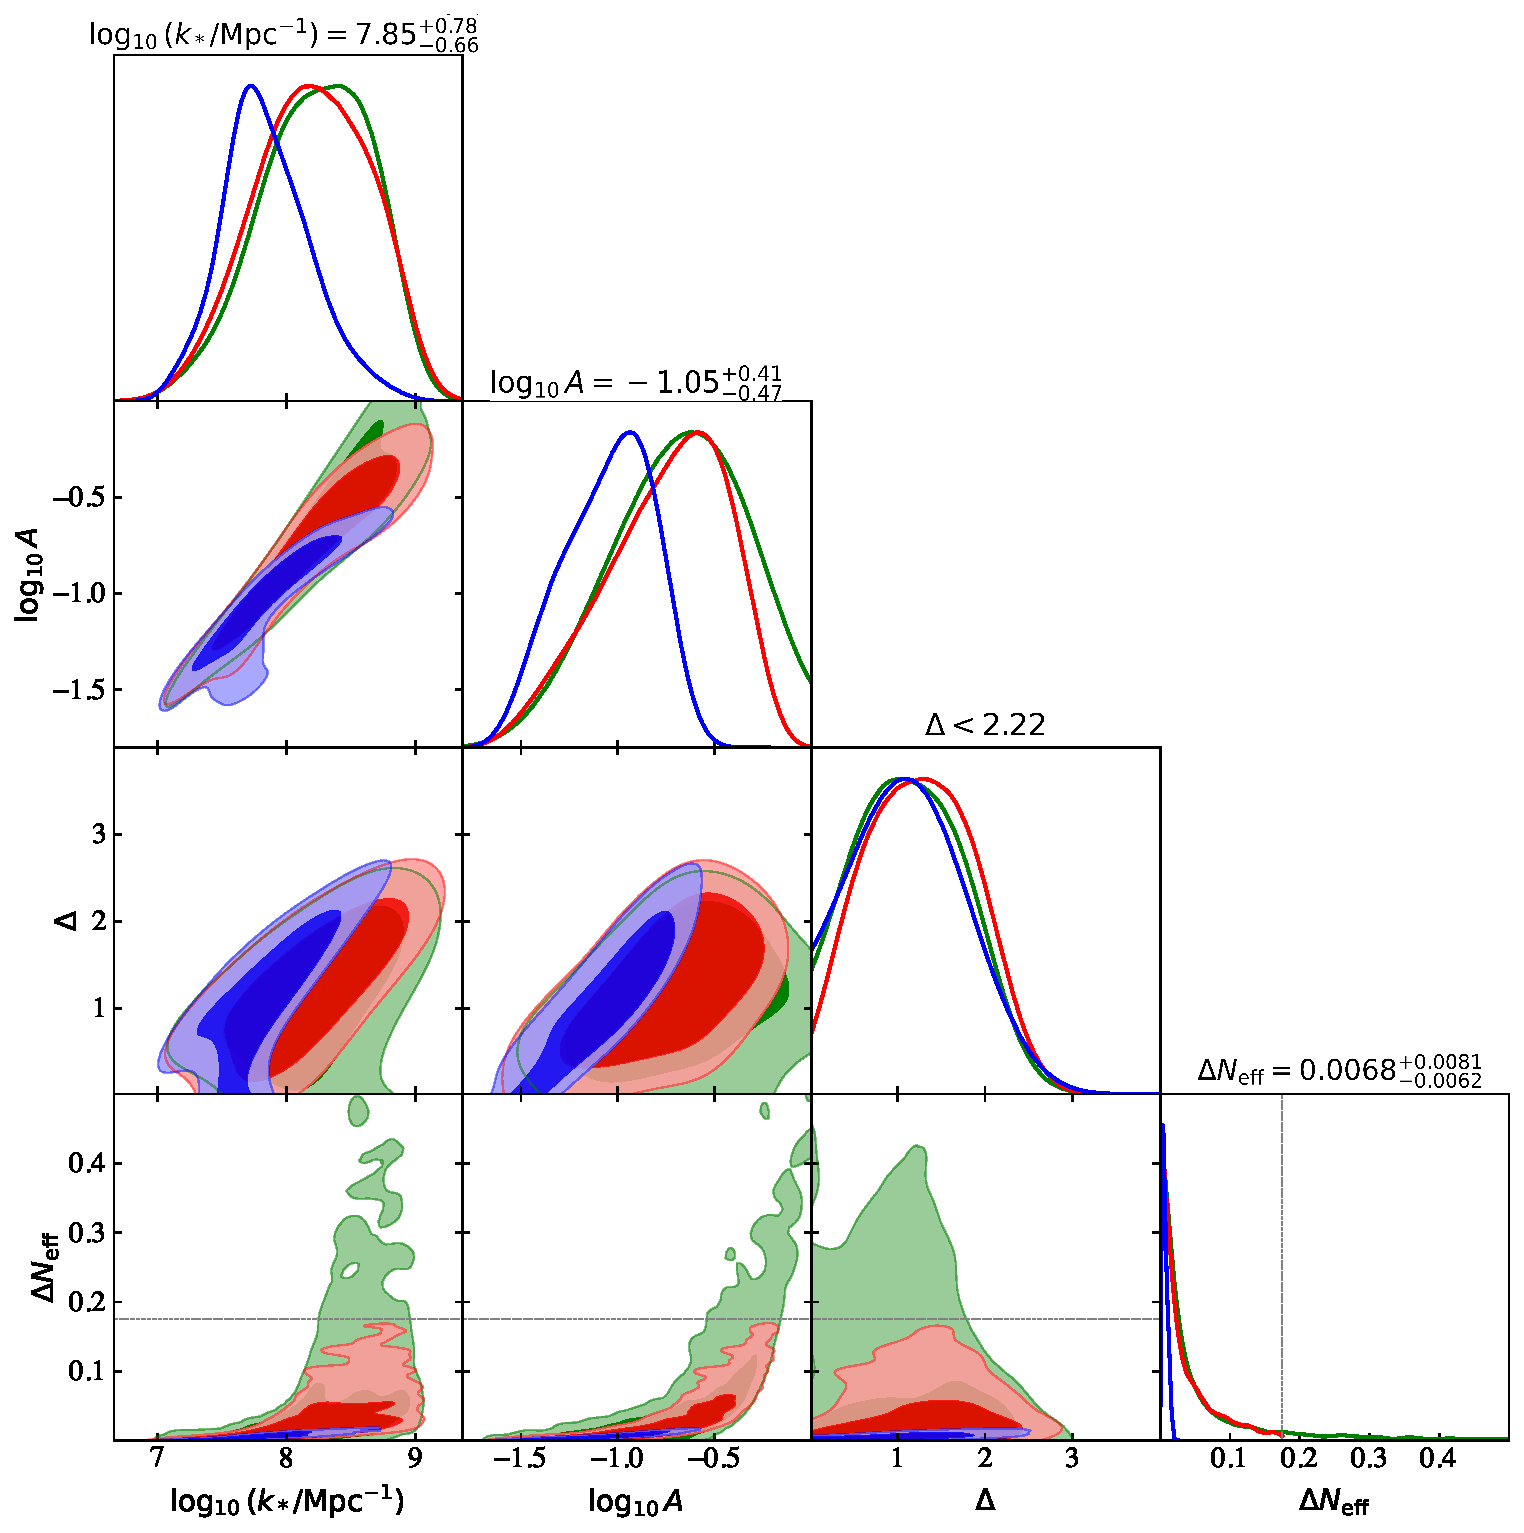
\includegraphics[width=8.5cm]{figs/param_posteriors.pdf}} \subfigure{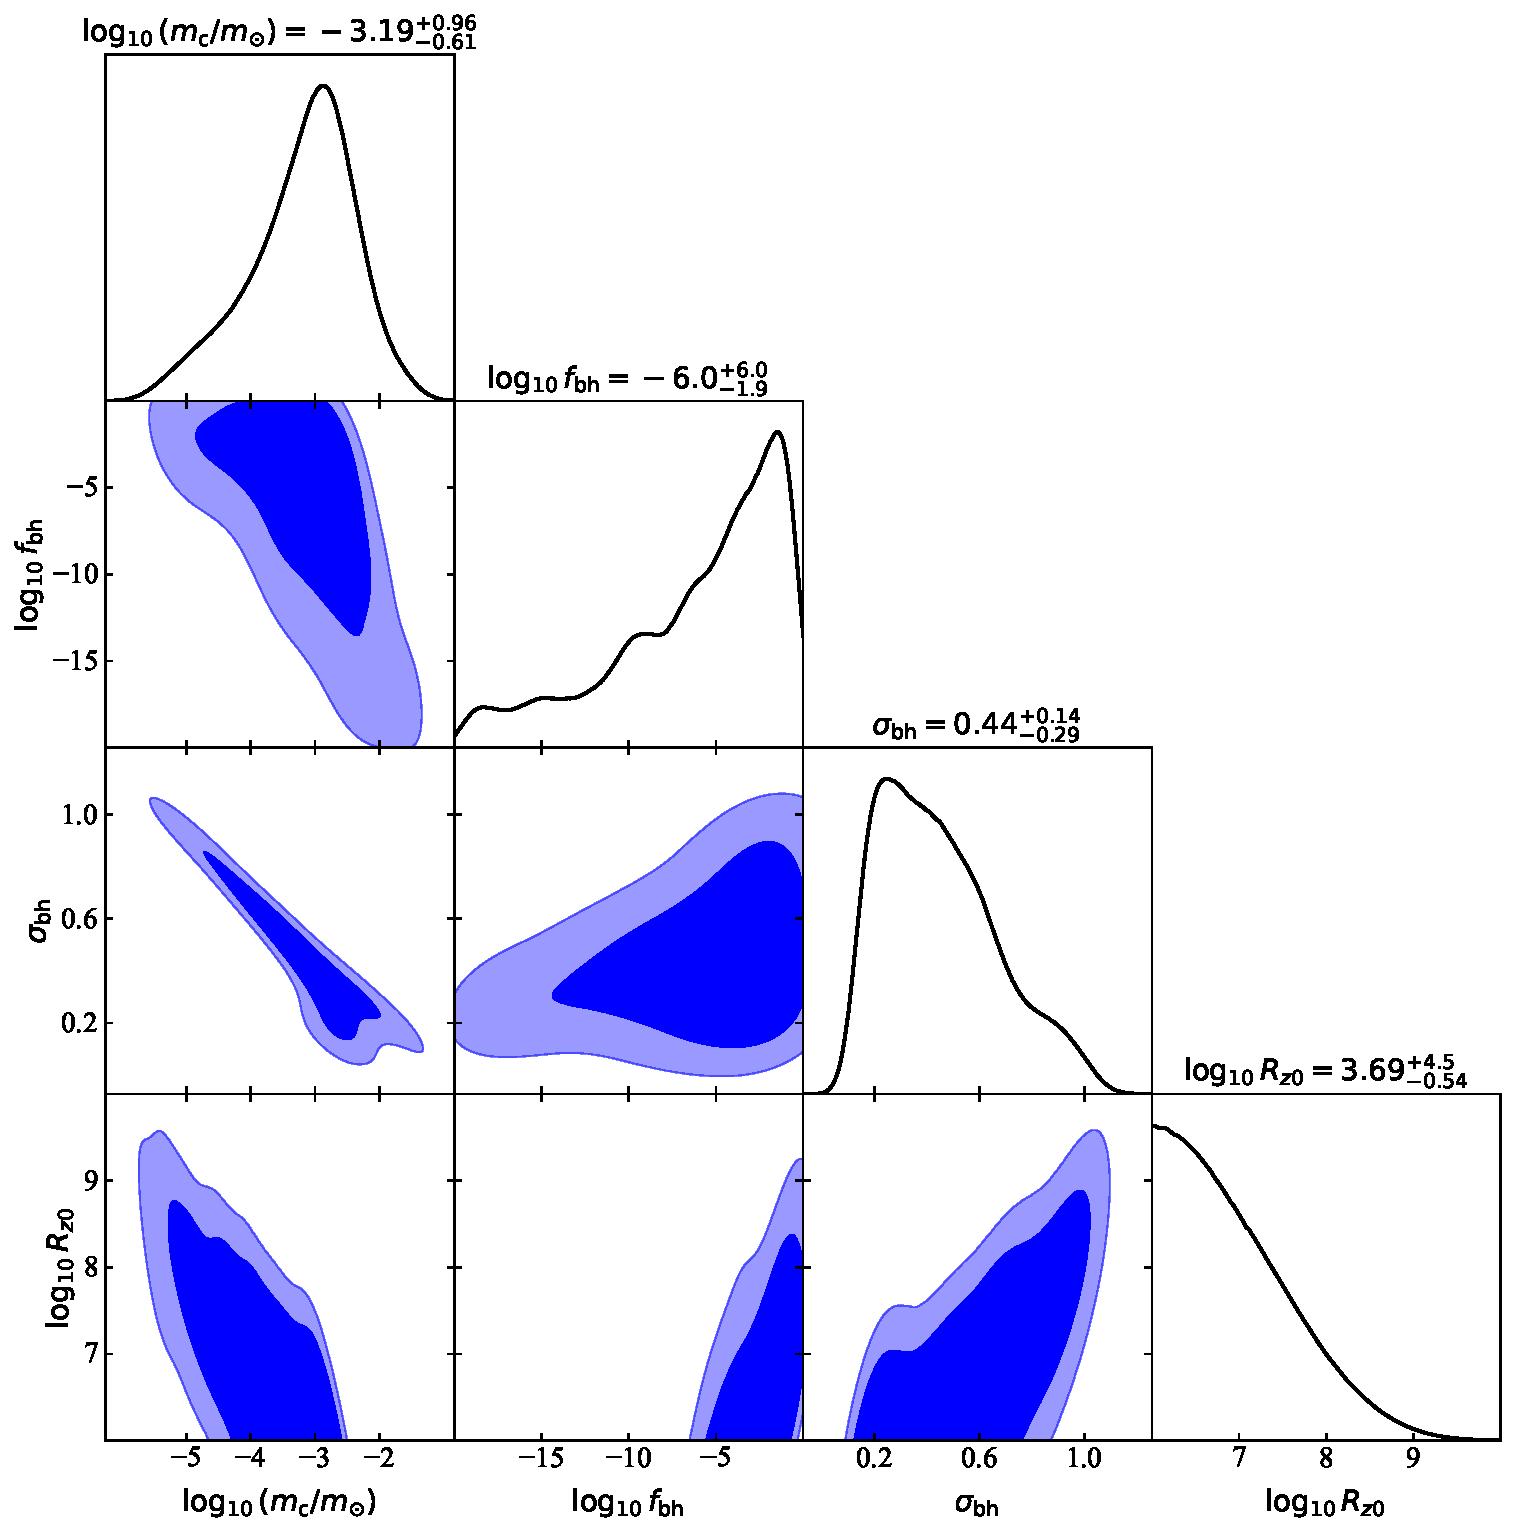
\includegraphics[width=8.5cm]{figs/PBH_posteriors.pdf}}\\
\caption{
{\bf Left}: marginalised posteriors for our model parameters and the derived $\dneff$,
the green (GW) posteriors show the result using GW data alone,
in the red (GW+$\dneff$) posteriors we used the GW data and the CBB limits on $\dneff$,
and the blue (GW+$\dneff$+PBH) posteriors show the results using GW data, CBB $\dneff$ constrains and the PBH prior of $\fbh \in [10^{-20},1]$.
The dotted line in the $\dneff$ panels indicates the value of $\dneff = 0.175$,
numbers on the diagonal panels show the marginalised mean and 68\% confidence region from GW inference.
{\bf Right}: posterior for PBH parameters $\fbh$, $m_\r{c}$, $\sigma_\r{bh}$ and merger rate $R$ (at $z=0$, in $\r{Gpc^{-3}yr^{-1}}$ unit),
derived from the GW+$\dneff$+PBH inference on the left panel,
numbers on the diagonal panels show the marginalised mean and 68\% confidence region from GW+$\dneff$+PBH inference.
}
\label{e2ftssaasadwu}
\end{figure*}

\begin{figure*}[htp]
\centering
\subfigbottomskip=-500pt
\subfigure{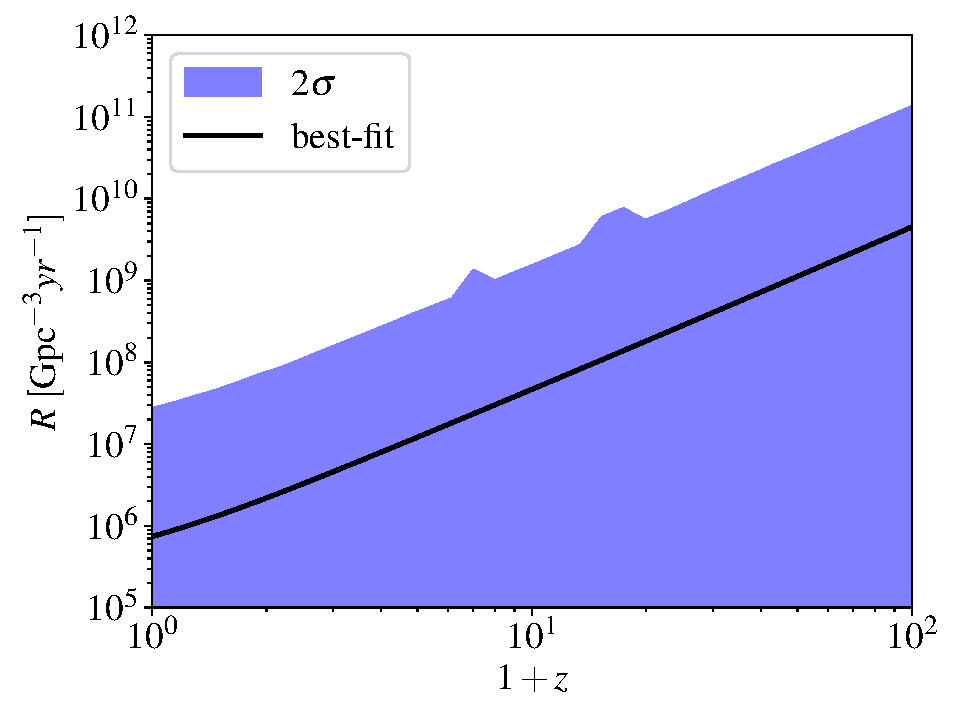
\includegraphics[width=8.5cm]{figs/Merger_rate_posteriors.pdf}} \subfigure{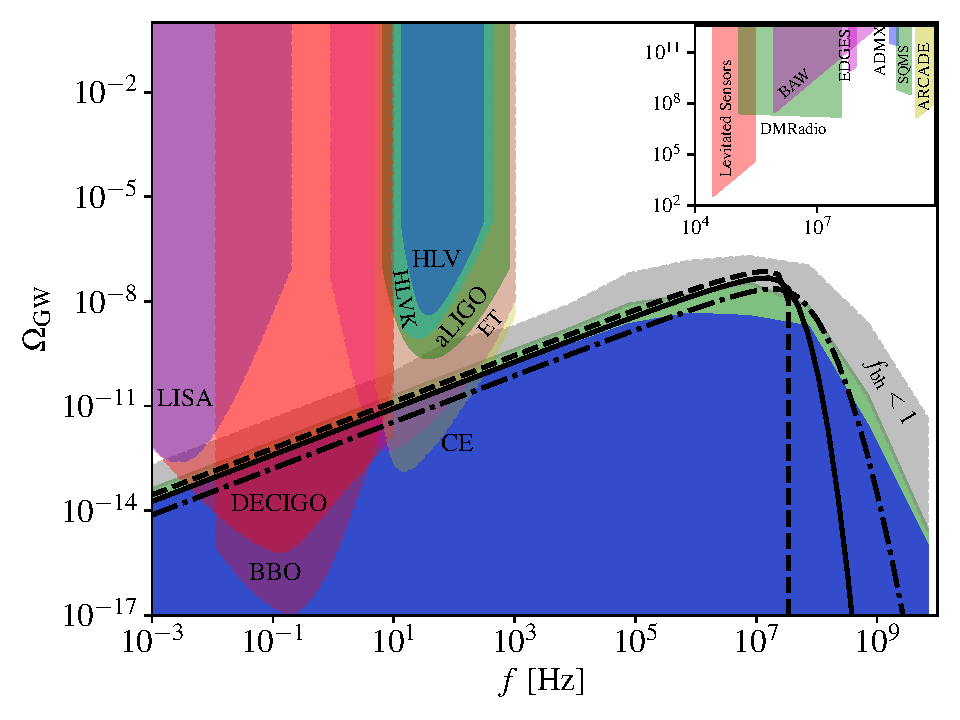
\includegraphics[width=8.5cm]{figs/Merger_GW_posteriors.pdf}}\\
\caption{
95\% C.L. confidence region for merger rate (left) and merger $\Omega_\r{GW}$ (right),
the solid black line in both panels correspond to PBH parameters values $\fbh = 10^{-2},\ m_\r{c} = 10^{-3}m_{\odot},\ \sbh = 0.1$,
which roughly corresponds to the best-fit values from our inference.
The grey shaded regions on the right panel show the expected experimental sensitivity of xxxxxxxx.
}
\label{e2f8nb_asadwu}
\end{figure*}

\section{Discussion}

\bigskip

{\bf Acknowledgements.}~~


\begin{appendix}
\label{apdsaSpecs}
\onecolumngrid
\section{Mass functions}
Let's define 
\be
\Psi
\equiv
\frac{\rd n_\r{bh}}{n_\r{bh} \rd \ln \mbh}
\label{Nodsfye4yuefg}
\ee
and
\be
\Phi
\equiv
\frac{\rd \rho_{\r{bh}}}{\rho_{\r{bh}} \rd \mbh}
=
\frac{\rd n}{\rho_{\r{bh}} \rd \ln \mbh}
\label{dwuh378yfhj}
\ee

Note that \Eq{Nodsfye4yuefg} and \Eq{dwuh378yfhj} are conventions used in 2012 and 1812 respectively.
It can be easily shown that $\Psi$ is related to $\Phi$ by
%\be
%\Psi
%=
%\frac{\rho_\r{bh}}
%{n_\r{bh}}
%\Phi
%\ee

\be
\Psi
=
P
\Phi
,\ 
P
=
\frac{\rho_\r{bh}}
{n_\r{bh}}
=
\left[
\int \frac{\rd \mbh}{\mbh}
\Phi
\right]^{-1}
\ee

In accordance with 2012,
let's further define the average of any quantity $F$ by,
\be
\left<F\right>
\equiv
\int \rd \ln \mbh
F
\Psi
\ee

Expressing this equation in terms of $\Phi$,
we get
\be
\left<F\right>
=
P
\int \rd \ln \mbh
F
\Phi
\ee

In the context of the mass function of this work,
$\Phi$ is given by,
\be
\Phi
=
\frac{1}{\sqrt{2 \pi} \sbh \mbh}
\exp
\left[
-
\frac{\r{ln}^2(\mbh/m_{\r{c}})}
{2 \sbh^2}
\right]
\ee
and $P$ can be solved analytically
\be
P
=
\left<
m\right>
=
m_\r{c}
\r{e}^{-\sbh^2/2}
\ee







\end{appendix}

\bibliography{refs.bib}

\end{document}




